\documentclass [9 pt]{article}
\usepackage[margin = 1in]{geometry}
\usepackage{amsfonts}
\usepackage{amsthm}
\usepackage{bbm}
 \usepackage{amsmath}
\usepackage[utf8]{inputenc}
\usepackage{graphicx}
\usepackage{enumerate}
\usepackage{color}
\usepackage{graphicx}
\graphicspath{ {./images/} }

\theoremstyle{definition}
\newtheorem{problem}{Problem}
\newtheorem{theorem}{Theorem}
\newtheorem*{corollary}{Corollary}
\newtheorem{proposition}[theorem]{Proposition}
\newtheorem{lemma}[theorem]{Lemma}
\newtheorem{conjecture}[theorem]{Conjecture}

\newtheorem{definition}[theorem]{Definition}
\newtheorem{remark}[theorem]{Remark}
\newtheorem{example}[theorem]{Example}


\usepackage{fancyhdr}
\pagestyle{fancy}
\lhead{Yuhao Wu \quad 260711365} 
\rhead{\bfseries COMP 330}
\cfoot{\thepage}
\renewcommand{\headrulewidth}{0.4pt}
\renewcommand{\footrulewidth}{0.4pt}

\setlength{\parindent}{0pt}



\begin{document}

\title{COMP 330}
\date{2018-9-05}
\author{Name: Yuhao Wu\\
ID Number: 260711365
}
\maketitle

\section*{Relations:}
correspondence of elements of two sets:\\
EXAMPLE: Two sets $A$ and $B$, $R \subseteq A \times B \quad \text{(Cartesian product)}$ \\
NOTE: R stands for "Relationship"

\begin{itemize}
	\item not every elements in $A$ needs to be related to anything in $B$
	\item A given element in $A$ could be several things in $B$
	\item When every element of $A$ is related to exactly one element in $B$ we get a function
\end{itemize}

\section*{Equivalent Relations:}
R is an equivalent relation on a set $S$, $R \subseteq S\times S $
\begin{itemize}
	\item $\forall s \in S$, $s-R-s\quad \quad \quad (reflexive)$ 
	\item $\forall s, t \in S$, $s-R-t \implies t-R-s\quad \quad \quad (symmetric)$
	\item $\forall s, t, p \in S$, $ s-R-t, t-R-p \implies s-R-p \quad \quad \quad (transitive) $
\end{itemize}
EXAMPLE: $ n \equiv m  $ (natural numbers) (mod 5) $\implies 32 \equiv 27 (mod \quad 5)$\\
\newline
\textbf{Definition:} Given an equivalence relation $R$, an equivalence class of an element x\\
$$\bigg[x\bigg] = \bigg\{ y | x-R-y \bigg\} $$
EXAMPLE: $[2] = \{ 7, 12, 17, 22, \ldots \} \quad \quad [2] = [7] $\\
FACT: Two different equivalence class can't have any elements in common

\section*{Partial Order:}
\textbf{Definition:} a binary relation $\quad \quad \quad \leq (\text{ less than or equal to  }) \quad \quad \quad < (\text{ strictly less than })$\\
\newline
\textbf{Axioms:}
\begin{itemize}
	\item $\forall s\quad s \leq s$\\
	\item $\forall s \text{ and } t,\quad s \leq t, t \leq s \implies s = t$\\
	\item $\forall s,  t, \text{ and } r, \quad s\leq t \text{ and } t\leq r \implies s \leq r$
\end{itemize}
\newpage
\textbf{REMARK:}
\begin{itemize}
	\item It might happen that two elements can not be compared.
	\item If every pairs can be compared, which means that:
	$$ \forall s \text{ and } t, s \leq t \text{ or } t \leq s \implies \text{ (total order) } \quad \quad \text{[this doesn't always hold]}$$
\end{itemize}
\textbf{EXAMPLE 1:}\\
$\{a, b, c\}$\\
All the subset of ${a, b, c} \implies \emptyset, \{a\}, \{b\}, \{c\}, \{a, b\}, \{a, c\}, \{ b, c\}, \{a, b, c\} $ \\
\bigg[ the power set (or powerset) of any set $S$ is the set of all subsets of $S$ \bigg]
$$ \{ a \} \subseteq \{ a, b \} \subseteq \{ a, b, c \}  \quad \big[ \text{this can be compared} \big]\quad \quad \quad \{ a, b\} \text{ and } \{a, c\}  \quad \big[\text{this can't be compared} \big]  $$
\newline
\textbf{EXAMPLE 2:}\\
$$natural \quad \mathbb{N}\quad \quad \quad real \quad \mathbb{R}\quad \quad \quad integer \quad \mathbb{Z}    $$
\newline
\textbf{EXAMPLE 3:}\\
$ f: \mathbb{R} \to \mathbb{R} $\\
Define: $ f \leq g \text{ [order of function] } \quad  if \quad \forall r \in \mathbb{R}, f(r) \leq g(r) \text{ [ order of numbers (numerical orders) ] }   $\\
This is not total order $\implies [\sin(x) \text{ and } \cos(x)]$ 

\section*{Well-Founded-Order:}
\textbf{Minimal VS Least:}
\begin{itemize}
	\item Minimal: there is nothing smaller than $x$ (strictly)
	\item Least: $x$ is smaller than anything else 
\end{itemize}
\textbf{NOTE:} there may be multiple different element to be \textbf{Minimal} due to incomparability.\\
\newline
\textbf{EXAMPLE:} \\
$$U_1 = \{ \{ a, b \}, \{ a, c \} , \{ a\} \} \implies \text{ least element is } \{ a \}$$
$$U_2 = \{ \{ a, b \}, \{ a, c \} , \{ a\}, \{ b \} \} \implies \text{2 least element is } \{ a \}, \{ b \}$$
\newline
\textbf{REMARK:} Least element is always the minimal\\
\newline
\section*{Well-Foundedness: $W$(set), $(W, \leq)$ }
\textbf{Definition: } For every non-empty subset $U$ of $W$, $(U \neq \emptyset \quad \&\&\quad U \subseteq W)$, $\exists u_0 \in U $ such that $u_0$ is minimal in $U$.\\
\newline
\textbf{EXAMPLE:} 
\begin{itemize}
	\item $(\mathbb{N}, \leq)$ is well-founded\\
	\item $(\mathbb{R}, \leq)$ is not well-founded $\quad$  as you can't find the minimal \\
\end{itemize}
\newpage
\textbf{NOTE:}
\begin{itemize}
	\item A well-founded total order is called a well-order\\
	\item If an order is not well-founded, there are infinitely long strictly descending sequence\\
	\item Induction works if your order is well-founded.
\end{itemize}
$$ \text{ well-founded } \implies \text{partial order} + \text{ exists minimal  } $$
$$ \text{ well-founded } + \text{total order} \implies \text{well order} $$

\section*{Induction: }
Suppose that $(S, \leq)$ is a poset, we say that the principle of induction holds for $S$ if for any predicate $P$ , we have
$$\bigg[ \forall x \in  S, ( \forall y \in S, y < x \implies P(y)) \implies P(x) \bigg] \implies \forall x \in  S, \quad P(x) $$\\
\textbf{Theorem: } An order is inductive if and only if it is well-founded.
\begin{proof}
	Assume that $(S, \leq)$ is well-founded. Suppose that $P(.)$ is any predicate.\\
	And suppose that $\forall x \in  S, ( \forall y \in S, y < x \implies P(y)) \implies P(x) $\\
	then we need to prove that $\forall x \in S, P(x)$\\
	Let $U = \bigg\{x\in S | \neg P(x) \bigg\} \quad \quad \text{suppose that there is one element in S such that P(x) is false}$\\
	Then we need to prove that $U = \emptyset $ \\
	\newline
	Suppose that $U \neq \emptyset \quad \quad \text{prove by contradiction}$\\
	As it is well-founded, there must be a minimal element $u_0$ in U\\
	$ \forall y \leq u_0, y \in S \implies y \notin U \quad \quad \text{ as $u_0$ is the minimal element in $U$, $y \leq u_0$, this is obviously, it is not in $U$ } $\\
	Then for $\forall y \in S, y \notin U \implies P(x)$\\
	Then, we use the assumption, $\forall x \in  S, ( \forall y \in S, y < x \implies P(y)) \implies P(x) $, \\
	as we can see that $u_0 \in S, and, y < u_0  $, so we can say that $P(u_0)$ holds $\implies u_0 \notin U \implies U = \emptyset$.\\
	Thus, we can conclude that $\forall x \in S, P(x)$
	
	
\end{proof}

\section*{Language recognition:}
Alphabet: $\Sigma = \{a, b, c \} \text{ or }\Sigma = \{0, 1 \} \implies  $ a finite set of symbols\\
Word: a sequence of letters  $\implies $ need to be finite length
\\
\newline
\textbf{EXAMPLE: }\\
Fix $\Sigma = \{a, b \}$, a word can be $a, ab, abb, baba, \ldots$
\begin{itemize}
	\item An empty word: $\epsilon$
	\item The collection of all words constructed by $\Sigma$ is denoted as $\Sigma^{*} \implies infinity $  
	\item A language $L \subseteq \Sigma^{*}$
\end{itemize}
\textbf{REMARKS:}
\begin{itemize}
	\item $L  = \emptyset $ (empty language) $\neq$ $L = \{ \epsilon \}$ (a word but an empty word )
	\item $L$ may be finite or infinite
\end{itemize}
\newpage
\textbf{NOTE:}\\
We need a notation to describe a language, we need algorithm to check if a word is in a certain language.\\
EXAMPLE: $L = \{w | \text{L has equal number of a and b} \}$

\section*{DFA: Deterministic Finite Automata}
A DFA is a 4-tuple:
\begin{itemize}
	\item $S := $ a finite set of states
	\item $S_0 \in S :=$ initial state
	\item $\delta  $(transition function) $\quad \quad \delta: S\times \Sigma \to S$ 
	\item  $F \subseteq S$ accepting states 
\end{itemize}

\textbf{Definition: } A language recognized by \textbf{DFA} is called a \textbf{Regular language}\\
\textbf{Remark: } Every state must have an arrow for every letter of $\Sigma$
\\
\newline
\textbf{Proposition: }
\begin{itemize}
	\item Every finite language is regular.
	\item It is possible to have some states that can't be reached.
\end{itemize} 

\textbf{Definition: }\\
$\delta^{*} : S \times \Sigma \to S$\\
\newline
Inductive Definition:\\
$\delta^*(s, \epsilon ) = s $\\
$\delta^*(s, aw ) = \delta^*( \delta(s, a) , w ) $\\
\newline
\newline
Formal definition of a DFA machine: $L(\mathbb{M}) = \{w\in \Sigma^*|\delta^*(s0, w) \in F\}$\\
\newline
\newline
\textbf{Definition:}
A language recognized by a DFA is called \textbf{Regular Language}

\subsection*{DFA Example:}
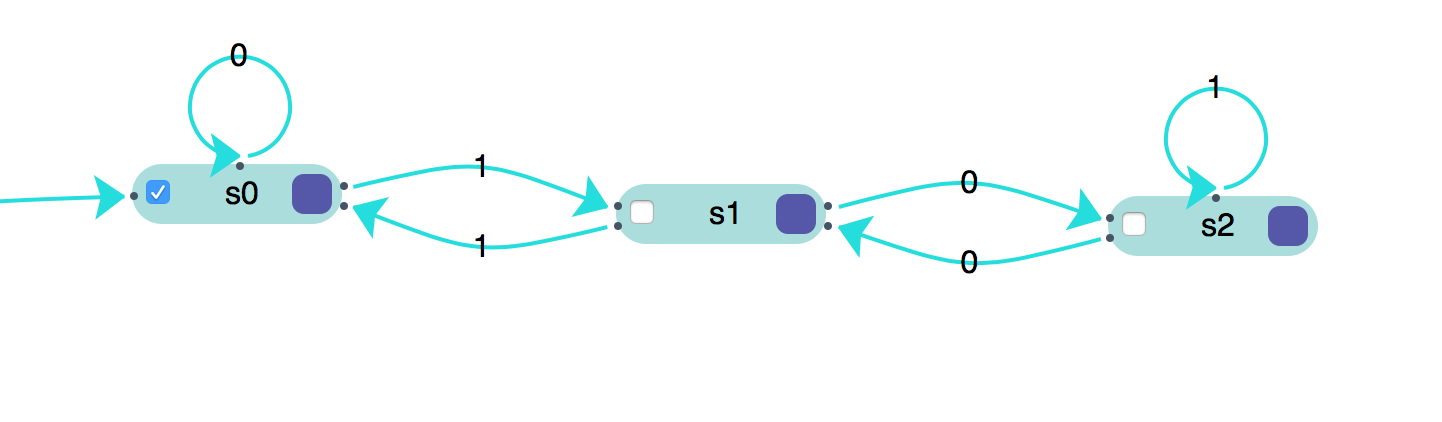
\includegraphics[scale=0.7]{1.png}
$$\Sigma = \{ 0, 1\}\quad\quad \text{Accept: multiple of 3 in binary number forms}$$
Read and scan numbers\\
\textbf{NOTE:} DFA won't know what previous number is, it can only read current number and make decisions according to the current number.\\
\textbf{Explanation: } There are three states: \\
$S_0 $ means the remainder is 0, if the next input is 0, which means $x = 2\times x \implies $ the remainder is 0 as well.\\
If the next input is 1, which means $x = 2\times x + 1$, the remainder is 1, so go to state $S_1$\\
\newline
\textbf{REMARKS:}
\begin{itemize}
	\item Any machine does this job needs at least 3 states.\\
		  There is a unique smallest machine for every language\\
	\item Suppose that we have a machine which has only two states and can do the job as well.\\
		  We must has one accept state and one reject state. \\
		  Obviously, 100 and 101 belongs to the same state, we add 1, get 1001 and 1011, which leads to different states.
\end{itemize}
\section*{NFA: Nondeterministic Finite Automaton}
How to design a machine accepting string ending in "aa".\\
There is an algorithm which converts any NFA to its equivalent DFA.\\
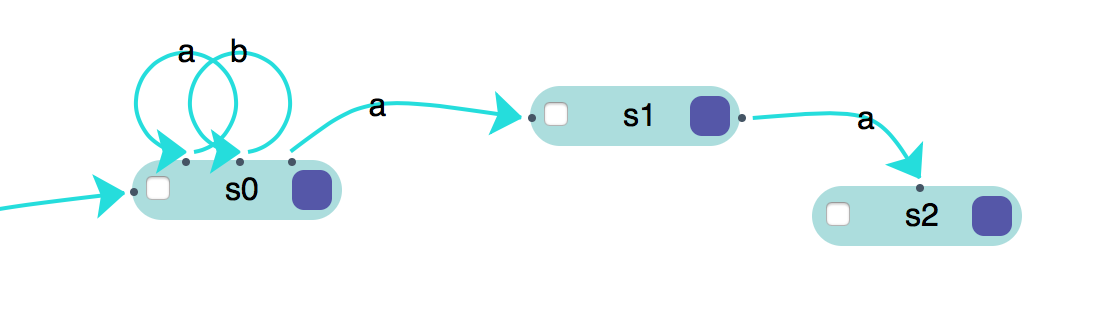
\includegraphics{2.png}
They recognize the same language: EXAMPLE: $"baabbaa"$\\
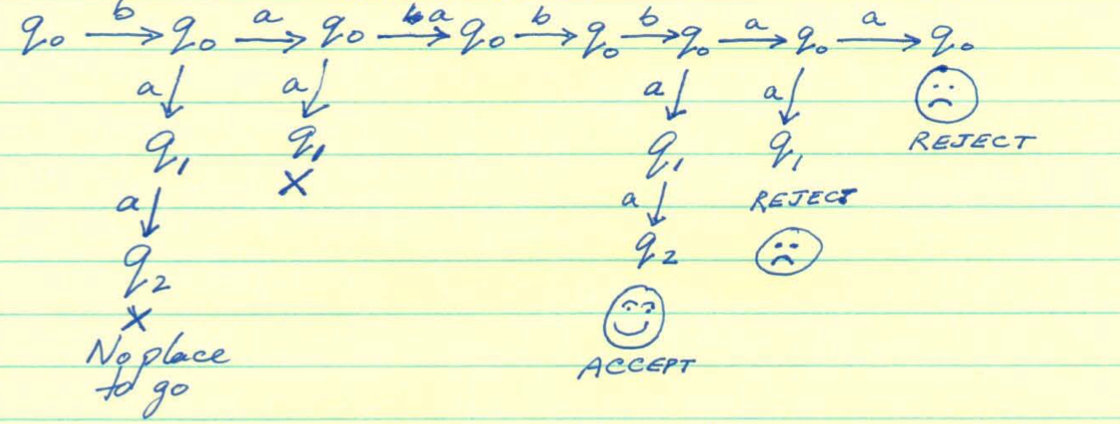
\includegraphics[scale = 0.8]{3.png}\\
It doesn't matter that some path going into rejected state as long as there is one path goes to accepted state.
\subsection*{NFA + $\epsilon$: Jump without reading a word: }
$\Sigma = \{. , + , -, 0, 1,\ldots ,9 \}$\\
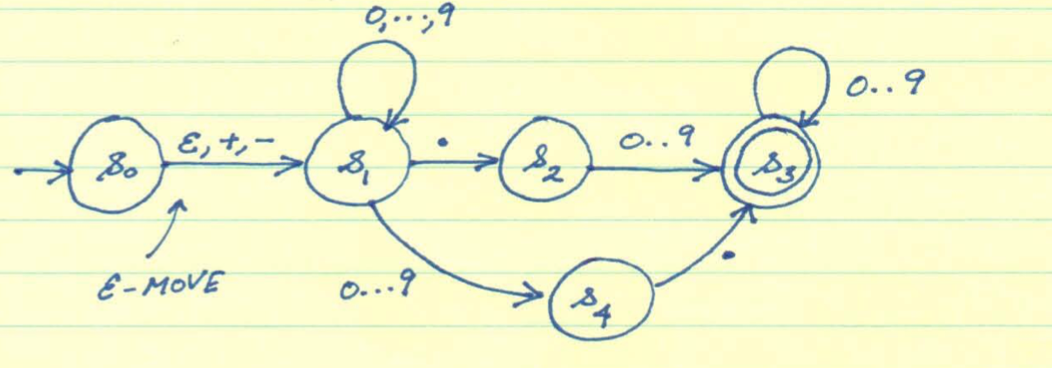
\includegraphics{4}\\




\end{document}